\documentclass[a4paper, 12pt]{article}
\usepackage[margin=1in]{geometry}
\usepackage[english, ngerman]{babel}
\usepackage[autostyle]{csquotes}
\usepackage{natbib}

% \bibliographystyle{ksfh_nat}
% \bibliographystyle{apa}
\bibliographystyle{apalike}
% \bibliographystyle{plainnat}

\usepackage{hyperref}
\usepackage{graphicx}
\usepackage{titlesec}
\usepackage{subcaption}
% \usepackage[raggedrightboxes]{ragged2e}
% \usepackage{pgf-pie}
% \usepackage{pgfplots}
\usepackage[acronym, toc, numberedsection]{glossaries}
\usepackage{listings}
\usepackage{amsmath}

\lstdefinelanguage{JavaScript}{
  keywords={typeof, new, true, false, catch, function, return, null, catch, switch, var, if, in, while, do, else, case, break, const, let},
  ndkeywords={class, export, boolean, throw, implements, import, this, string, number, date},
  sensitive=false,
  comment=[l]{//},
  morecomment=[s]{/*}{*/},
  morestring=[b]',
  morestring=[b]"
}
\lstdefinestyle{mystyle}{
    % backgroundcolor=\color{backcolour},   
    commentstyle=\color{teal},
    keywordstyle=\color{red},
    ndkeywordstyle=\color{blue},
    numberstyle=\footnotesize\color{gray},
    stringstyle=\color{violet},
    % basicstyle=\ttfamily\normalsize,
    % basicstyle=\ttfamily\small,
    basicstyle=\ttfamily\footnotesize,
    breakatwhitespace=true,         
    breaklines=true,                 
    captionpos=b,                    
    % keepspaces=true,                 
    numbers=left,                    
    % numbersep=5pt,                  
    showspaces=false,                
    showstringspaces=false,
    % showtabs=false,                  
    tabsize=2,
}
\lstset{style=mystyle}

\usepackage{hyphenat}
% \hyphenation{Mathe-matik wieder-gewinnen}
\usepackage[T1]{fontenc}
\usepackage[table]{xcolor}
\usepackage[export]{adjustbox}
\usepackage{multirow}
\usepackage{multicol}

\usepackage{newfloat}
\DeclareFloatingEnvironment[placement={!ht},name=List]{mylist}

\makenoidxglossaries
\newacronym{dom}{DOM}{Document Object Model}
\newacronym{html}{HTML}{Hypertext Markup Language}
\newacronym{css}{CSS}{Cascading Style Sheet}
\newacronym{js}{JS}{JavaScript}
\newacronym{json}{JSON}{JavaScript Object Notion}
\newacronym{csr}{CSR}{Client-side Rendering}
\newacronym{ssr}{SSR}{Server-side Rendering}
\newacronym{svg}{SVG}{Support Vector Graphic}
\newacronym{cicd}{CI/CD}{Continuous Integration and Continuous Delivery}
\newacronym{tbw}{TBW}{Total Byte Weight}
\newacronym{ttfb}{TTFB}{Time To First Byte}
\newacronym{tti}{TTI}{Time To Interactive}
\newacronym{tbt}{TBT}{Total Blocking Time}
\newacronym{lvc}{LVC}{Last Visual Change}
\newacronym{olvc}{OLVC}{Observed Last Visual Change}
\newacronym{lcp}{LCP}{Largest Contentful Paint}
\newacronym{fvc}{FVC}{First Visual Change}
\newacronym{ofvc}{OFVC}{Observed First Visual Change}
\newacronym{ovcd}{OVCD}{Observed Visual Change Duration}
\newacronym{seo}{SEO}{Search Engine Optimization}
\newacronym{pwa}{PWA}{Progressive Web App}
\newacronym{cli}{CLI}{Command Line Interface}
\newacronym{url}{URL}{Uniform Resource Locator}
\newacronym{http}{HTTP}{Hypertext Transfer Protocol}

\title{Mega-fast or just super-fast? Performance differences of mainstream JavaScript frameworks for web applications}
\author{Andreas Nicklaus}

\makeatletter

\renewenvironment{thebibliography}[1]
     {\section{References}
      \@mkboth{\MakeUppercase\bibname}{\MakeUppercase\bibname}%
      \list{\@biblabel{\@arabic\c@enumiv}}%
           {\settowidth\labelwidth{\@biblabel{#1}}%
            \leftmargin\labelwidth
            \advance\leftmargin\labelsep
            \@openbib@code
            \usecounter{enumiv}%
            \let\p@enumiv\@empty
            \renewcommand\theenumiv{\@arabic\c@enumiv}}%
      \sloppy
      \clubpenalty4000
      \@clubpenalty \clubpenalty
      \widowpenalty4000%
      \sfcode`\.\@m}
     {\def\@noitemerr
       {\@latex@warning{Empty `thebibliography' environment}}%
      \endlist}

\renewcommand\listoffigures{%
  \section{\listfigurename}%
  \@mkboth{\MakeUppercase\listfigurename}{\MakeUppercase\listfigurename}%
  \@starttoc{lof}%
}
\renewcommand\listoftables{%
  \section{\listtablename}%
  \@mkboth{\MakeUppercase\listtablename}{\MakeUppercase\listtablename}%
  \@starttoc{lot}%
}
\renewcommand\lstlistoflistings{
  \section{\lstlistlistingname}
  \@starttoc{lol}%
}
\let\Title\@title
\let\Author\@author

\rowcolors{1}{lightgray!40!}{white}

% Keywords command
\providecommand{\keywords}[1]
{
  {
    \footnotesize
    \textit{\textbf{Keywords ---} #1}
  } 
}

\makeatother

\begin{document}

\begin{center}
  
\includegraphics[width=100px, keepaspectratio]{img/hdm-logo.png}
\end{center}	
  
\vspace{20px}
\noindent{\Large\bfseries \Title}
\vspace{10px}

\noindent\textbf{\Author}\\
Hochschule der Medien Stuttgart\\
an067@hdm-stuttgart.de 

\vspace{10px}
\noindent Prof. Dr. Fridtjof Toenniessen \& Stephan Soller

\selectlanguage{english}
\begin{abstract}
  An essential initial step in every modern web application project is the selection of an appropriate web development framework.
  Often, detrimental decisions are made based on sentiment rather than a proper assessment of the framework's performance vs. the project requirements and resources.

  This thesis presents a study of a model web application created identically with seven mainstream JavaScript web development frameworks: Angular, Astro, Next.js, Nuxt, React, Svelte and Vue.js.

  Performance measurements are done with Lighthouse and Playwright tools to identify strengths and weaknesses of the frameworks.
  To this end, classic page load times and the load and update times of JavaScript components are retrieved among other data.
  Additionally two new suitable derivative metrics are evaluated: the \enquote{Observed Visual Change Duration} and a "loadEventEnd" metric.

  The results show no clear-cut general advantage of a single web development framework.
  Component update times indicate Nuxt as the fastest web development framework.
  Next.js is the slowest one in this context.
  Similarly, Google Chrome appears to be the fastest client browser.
  Desktop Safari is the slowest one for updating the DOM after user input.
\end{abstract}

% \tableofcontents
% \pagebreak

% TODO: Ort der Tabellen und Bilder anpassen

\section{Introduction}
% What is the current situation?
% What should be done?
% Why am I doing this?

With the evolution of the world wide web, development of websites reached a higher complexity, both of the page content and the functionality.
This complexity resulted in higher demand for technical sophistication in networking, hosting services and development tools.
Although modern frameworks provide technical advancements to increase the speed of page and content generation and arguably a better developer experience, there is no apparent way to objectively determine a \enquote{best framework} in terms of development ease and speed.

When it comes to user experience and perceived performance however, there are plentiful collections of metrics and criteria to choose from so as to determine the performance of websites, not frameworks.
The strife always is to somehow better the web site performance since it has a palpable influence on search engine results, user acceptance and ultimately project success.
Hence, there are business interests and financial incentives to invest resources into performance optimization \citep{webprophet,effectsofwebpagecontents}.
Past research, existing tools and guides give direction to optimize websites according to stakeholders' and users' expectations.
Yet in most cases, the only focus on specific websites or specific frameworks or give general advice.

The lack of research on the effect of the framework on website performance indicates a need for research on the topic.
Relying on marketing material for the choice of framework is questionable because most modern frameworks claim to be fast, easy to use and performance efficient.
This suggests that each would be a great choice.
Thus, comparing frameworks presents a challenge because no ideal set of metrics for this use case is apparent and there are no publicly accessible replicas of web applications built with different frameworks available.
Therefore, a comparative study between versions of the same website built with different web development frameworks is needed.
With this data, an informed choice might be made for projects in the future.

The goals of this thesis are to propose a set of metrics that allow comparing mainstream \acrfull{js} frameworks for web applications, to provide a comparative study between selected frameworks and to create a tool to compare the rendering performance a web page as a whole and of dynamic components within a page.

\section{Application and testing environment}
% What is the application?
% What frameworks are tested?
% What metrics are used?
% What tools can do that?

\textbf{Frameworks.} One of the choices for the setup of the study is which frameworks to implement the application in and compare.
The selected frameworks have to support the designed web application without the help of another tool or framework unless intended by the developers of the framework.
Plus, the frameworks have to use \acrfull{js}  in order to narrow down the scope of the study.
TypeScript frameworks are allowed because they support \acrshort{js} \citep{typescript}.

Basis for the framework selection are the rankings of most-used, most-liked and most-interesting web development frameworks and tools \citep{stateOfJs2023}.
The following frameworks were selected for this framework:

\begin{multicols}{4}
\begin{itemize}
  \item Angular
  \item Astro
  \item Next.js
  \item Nuxt
  \item React
  \item Svelte
  \item Vue.js
\end{itemize}
\end{multicols}

Others like Preact, Solid and Qwik were considered to be included in this study, but were dropped because of negative sentiment or low usage among developers that have experience with the tools.
\\

\textbf{Web application.} The web application used for this study is designed to be the subject of comparisons between frameworks.
Its look is derived from the Android app of Instagram \citep{instagram} and it has four pages (see figure \ref{fig:screenshots}).
The four pages cover three generally valid page types identified in the design process.
The About page is a \enquote{Static page} as it does not change its content after the initial response from the web server.
No additional data query is needed to build the finished \acrshort{dom} structure.
The Feed page and the Profile page are \enquote{Delayed pages}.
Their defining characteristic is that the \acrshort{dom} cannot be fully built from the initial \acrshort{html} document, but needs data queries to complete before all content can be displayed.
These data queries are triggered immediately after the initial page request.
The Create page is the only \enquote{Dynamic page}.
Its initial features indicate it being either a static or delayed page, depending on the implementation, and it has dynamic components that update through user input.
Mutations to the \acrshort{dom} are therefore not only triggered by the initial page request but a user interaction.
The time of such changes is therefore not predictable.

\begin{figure}[h]
  \begin{subfigure}{0.24\linewidth}
    \begin{center}
      
\includegraphics[width=\linewidth, height=0.3\textheight, keepaspectratio,frame]{img/ig-clone/Informationsseite.png}
    \end{center}
    \caption{About page}\label{subfig:about}
  \end{subfigure}
  \begin{subfigure}{0.24\linewidth}
    \begin{center}
      
\includegraphics[width=\linewidth, height=0.3\textheight, keepaspectratio,frame]{img/ig-clone/Feed.png}
    \end{center}
    \caption{Feed page}\label{subfig:index}
  \end{subfigure}
  \begin{subfigure}{0.24\linewidth}
    \begin{center}
      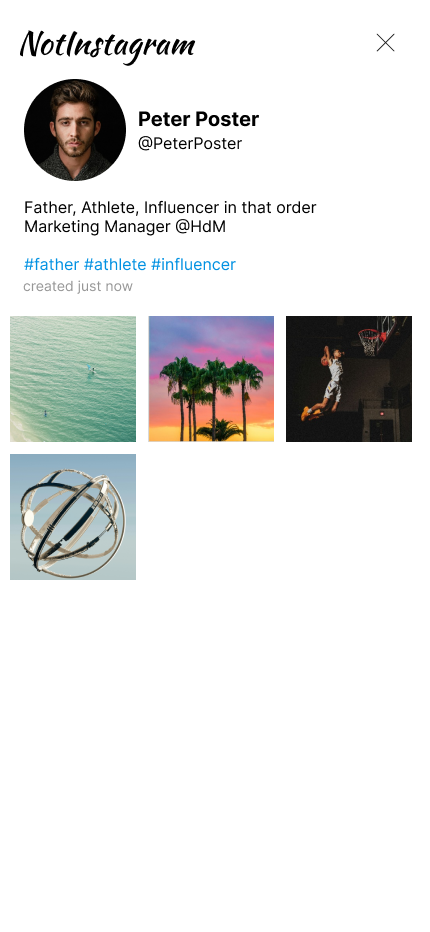
\includegraphics[width=\linewidth, height=0.3\textheight, keepaspectratio,frame]{img/ig-clone/Profil.png}
    \end{center}
    \caption{Profile page}\label{subfig:user}
  \end{subfigure}
  \begin{subfigure}{0.24\linewidth}
    \begin{center}
      
\includegraphics[width=\linewidth, height=0.3\textheight, keepaspectratio,frame]{img/ig-clone/Beitrag erstellen.png}
    \end{center}
    \caption{Create page}\label{subfig:create}
  \end{subfigure}
  \caption{Screenshots of the \enquote{NotInstagram} application's pages}\label{fig:screenshots}
\end{figure}

\textbf{Components.} These four pages are comprised of 15 components, most of which are wrappers to encapsulate image components, styled text or iterations over lists with subcomponents.
However, two components stand out because of their special purpose and implementation differences between frameworks.

\begin{enumerate}
  \item The MediaComponent is designed to present both internal and external image and video sources in a single component.
  It is used to display Profile images and Post content.
  Its main purpose is to decide - based on the passed source string - how to project the multimedia file onto the \acrshort{dom}.
  As such, a decision for enhanced image or video elements had to be made per framework during the implementation of the application.
  Svelte, Astro, Next.js and Nuxt provide such an enhanced image component.
  In contrast, video elements are inserted to the \acrshort{dom} as-is, but the browser behaviour is adapted identically for all frameworks using attributes on the \verb|<video>| element and \acrlong{js}.
  In addition, the import of local images differs between frameworks because the load behaviour differs.
  As such, some frameworks require importing all local images in order to select the requested image.
  \item Astro does not natively support dynamic components as needed in the Create page of the application.
  The intended solution is to implement so-called \enquote{Islands} using another framework.
  React is chosen for its high usage rate among web developers \citep{stateOfJs2023}.
  As a result, two implementations are compared in this study: Using the React components that are needed for Astro Islands everywhere, even if the component in question is not dynamic, and creating duplicate native Astro components for when a component is not required to be dynamic.
  One additional React component \enquote{CreateForm} was created in order to encapsulate React subcomponents and six components were implemented in React because they are part of the form and the Post preview on the Create page.
\end{enumerate}

\textbf{Hosting.} In order to test the end-products of the frameworks, at least one web server is needed to host the application.
Network delays are an obvious source of rendering and performance issues \citep{highperformancebrowsernetworking}.
For this reason, the tests for this study are performed on two different web servers: An online hosting service and the local testing machine.

\begin{enumerate}
  \item \textbf{Vercel} was chosen for hosting the applications on distant servers based on its popularity, capabilities for \acrfull{ssr}, support for both a free and paid version and its simple integration into \acrshort{cicd} pipelines.
  Each Vercel project was connected to a Github repository, one per framework.
  Only required project configuration options were changed per project on the plattform to ensure its state as \enquote{as-is}.
  \item A \textbf{local host} was chosen to minimize the effect of network delay and related delays, e.g. domain name resolving, in this study.
  The application is hosted on the testing machine.
  A HP Envy x360 with an AMD Ryzen 5 5500U processor and 16 GB RAM is used here.
  The OS on the device is Windows 11 Home (Version 10.0.22631) during testing.
  The application is built before every test and hosted using either built-in commands for the framework or using the \verb|serve| command. %(see table \ref{tab:hostCommands})
\end{enumerate}

% \begin{table}[h]
%   \begin{center}
%     \begin{tabular}[h]{| l | l | l |}
%       \hline
%       \textbf{Framework} & \textbf{Build Command} & \textbf{Host Command} \\ \hline
%       Angular & \verb|ng build| & \verb|serve| \\ \hline
%       Astro & \verb|astro build| & \verb|astro preview| \\ \hline
%       Next.js & \verb|next build| & \verb|next start| \\ \hline
%       Nuxt & \verb|nuxt build| & \verb|nuxt preview| \\
%       & \verb|nuxt generate| & \verb|nuxt preview| \\ \hline
%       React & \verb|react-scripts build| & \verb|serve| \\ \hline
%       Svelte & \verb|vite build| & \verb|vite preview| \\ \hline
%       Vue.js & \verb|vite build| & \verb|serve| \\ \hline
%     \end{tabular}
%   \end{center}
%   \caption{Build and host command for each used framework as used for testing the applications when hosted locally}\label{tab:hostCommands}
% \end{table}

\textbf{Metrics.} To identify strengths and weaknesses of the frameworks, eleven metrics were chosen to test the frameworks in three categories (see table \ref{tab:metriccategories}).
The Page Load Time (PLT) covers the classic load time of web pages and is specified to outline the load speed from \verb|requestStart| to the last change to the page.
The Component Load Time (CLT) is defined as the time frame in which any changes to the \acrshort{dom} with \acrshort{js} can be identified and the rendering process of \acrshort{js} components are shown.
The Component Update Time (CUT) is defined as the time between a user interaction and a \acrshort{dom} mutation.
This time frame describes the speed of feedback to the user that the interaction has been registered and something is happening as well as the speed until that something finishes happening.
Especially \acrshort{dom} mutation times are expected to show differences between frameworks and implementations as the \acrshort{html} elements and internal implementation change from one framework to another.

\begin{table}[h]
  \begin{center}
    \begin{tabular}[h]{|l|c|c|c|}
      \hline
                          & \textbf{PLT} & \textbf{CLT}  & \textbf{CUT}  \\ \hline
      \acrlong{tbw}       & x            &               &               \\ \hline
      \acrlong{ttfb}      & x            &               &               \\ \hline
      \acrlong{tti}       & x            & x             &               \\ \hline
      \acrlong{tbt}       & x            & x             &               \\ \hline
      LoadEventEnd        & x            & x             &               \\ \hline
      DomContentLoaded    & x            &               &               \\ \hline
      \acrlong{lvc}       & x            &               &               \\ \hline
      \acrlong{lcp}       & x            &               &               \\ \hline
      \acrlong{olvc}      &              & x             &               \\ \hline
      \acrlong{ofvc}      &              & x             &               \\ \hline
      DOM Mutation Times  &              & x             & x             \\ \hline
    \end{tabular}
    % \begin{tabular}[h]{|l|l|l|}
    %   \hline
    %   \multicolumn{1}{|c|}{\textbf{Page}}       & \multicolumn{2}{c|}{\textbf{Component}}     \\ \hline
    %   \multicolumn{1}{|c|}{\textbf{Load Time}}  & \textbf{Load Time}  & \textbf{Update Time}  \\ \hline
    %   \acrlong{tbw}                             & \acrlong{olvc}      &                       \\ \hline
    %   \acrlong{ttfb}                            & \acrlong{ofvc}      &                       \\ \hline
    %   \multicolumn{2}{|c|}{\acrlong{tti}}                             &                       \\ \hline
    %   \multicolumn{2}{|c|}{\acrlong{tbt}}                             &                       \\ \hline
    %   \multicolumn{2}{|c|}{LoadEventEnd}                              &                       \\ \hline
    %   DomContentLoaded                          & \multicolumn{2}{c|}{DOM Mutation Times}     \\ \hline
    %   \acrlong{lvc}                             &                               &             \\ \hline
    %   \acrlong{lcp}                             &                               &             \\ \hline
    % \end{tabular}
  \end{center}
  \caption{Assignment of metrics to the metric categories: Page Load Time (PUT), Component Load Time (CLT) and Component Update Time (CUT)}
  \label{tab:metriccategories}
\end{table}

\textbf{Test tools.} The requirements for testing tools - created by hosting the application on two different web servers and by the list list of metrics - are fulfilled by the Lighthouse CLI and Playwright.
They are set up so as to provide results both in human-readable and machine-readable format enabling easy debugging and automatic creation of aggregate metrics.
\\

\begin{enumerate}
  \item Using the \textbf{Lighthouse CLI}, a script for starting the web server and running Lighthouse tests on the web application is executed.
  These tests run 20 times and only cover the performance measurements of Lighthouse.
  Reports are created in both \acrshort{html} and \acrshort{json} format in order to debug the tests and create the mean average of every measurement.
  \item Tests with \textbf{Playwright} focus on the measurement of \acrshort{dom} mutations and the adherence to time budgets.
  To that end, a \acrshort{js} script is injected into the browser context before tests.
  This recording script initializes a MutationObserver on a specific \acrshort{html} element that is created by the framework.
  This way, all \acrshort{dom} mutations such as element addition, element removal and attribute change are recorded with an identifier of the element and the time of the mutation.
\end{enumerate}

The respective metrics covered by Lighthouse and Playwright are seen in table \ref{tab:metricassignment}.

\begin{table}[h]
  \begin{center}
    \begin{tabular}{|l|l|}
      \hline
      \textbf{Lighthouse} & \textbf{Playwright} \\ \hline
      \acrfull{tbw}       & domContentLoaded    \\ \hline
      \acrfull{ttfb}      & loadEventEnd        \\ \hline
      \acrfull{tti}       & User Input Times    \\ \hline
      \acrfull{tbt}       & Mutation Times      \\ \hline
      \acrfull{lcp}       &                     \\ \hline
      \acrfull{fvc}       &                     \\ \hline
      \acrfull{ofvc}      &                     \\ \hline
      \acrfull{olvc}      &                     \\ \hline
    \end{tabular}
  \end{center}
  \caption{Assignment of metrics to the test tools}
  \label{tab:metricassignment}
\end{table}

\section{Results}
% Page load times
% Component load times
% Component update times

Metrics for the page load and for the component load times show no clear generally applicable evidence for a single framework being faster than the others.
Such a distinction can only be made on a per-metric basis.
Figure \ref{fig:lighthouseResults} presents the averages of measurements from the Lighthouse reports per page and framework.
\\

% Lighthouse result graphs
\begin{figure}[!h]
  \centering
  \begin{subfigure}{0.49\linewidth}
    \begin{center}
      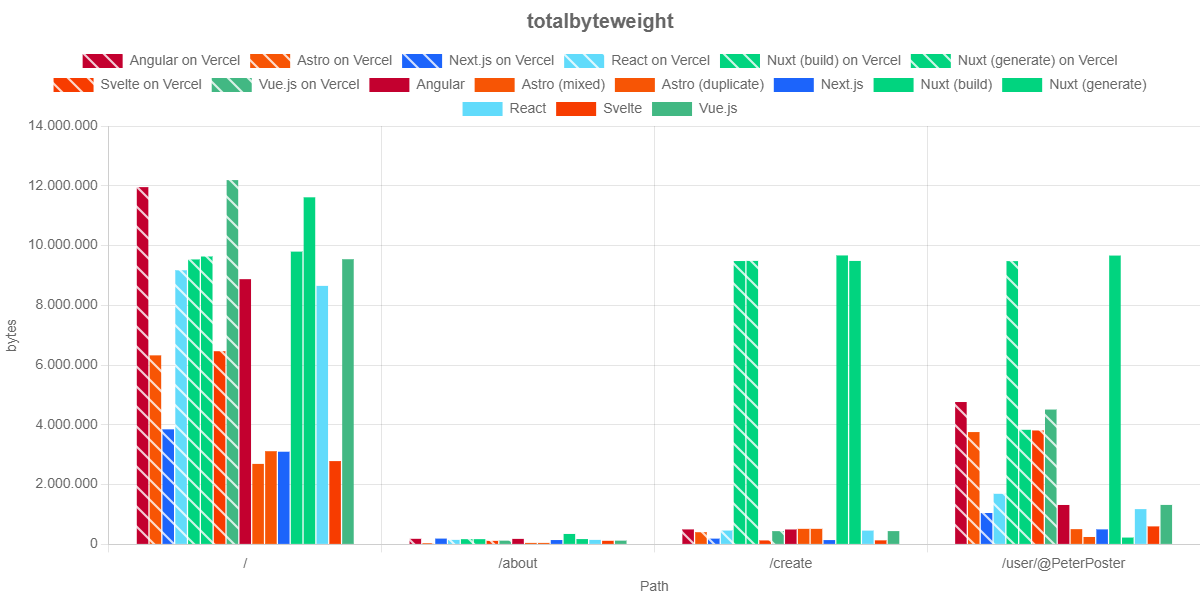
\includegraphics[width=\linewidth, keepaspectratio]{img/lighthouse-results/TBW.png}
    \end{center}
    \caption{\acrfull{tbw}}\label{subfig:LH:totalbyteweight}
  \end{subfigure}
  \begin{subfigure}{0.49\linewidth}
    \begin{center}
      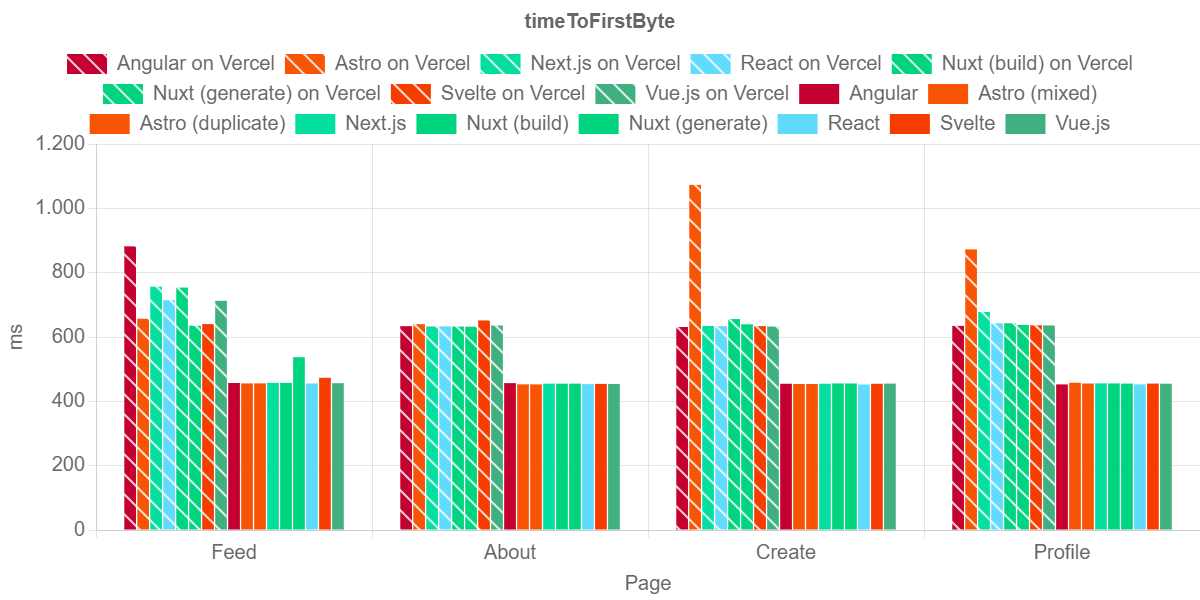
\includegraphics[width=\linewidth, keepaspectratio]{img/lighthouse-results/TTFB.png}
    \end{center}
    \caption{\acrfull{ttfb}}\label{subfig:LH:timeToFirstByte}
  \end{subfigure}
  \begin{subfigure}{0.49\linewidth}
    \begin{center}
      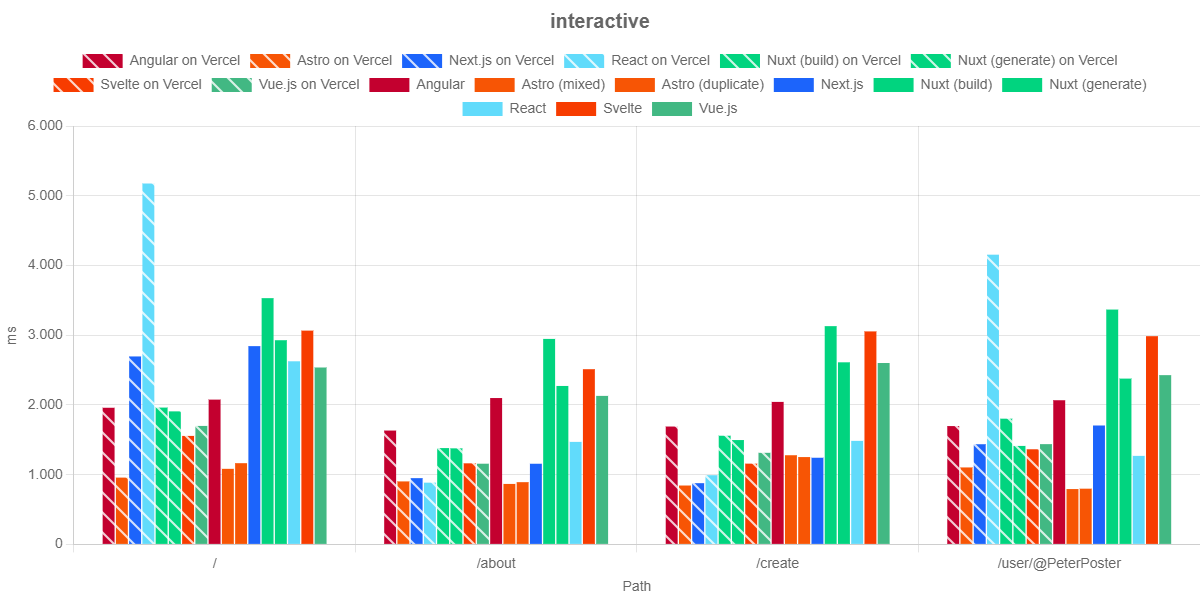
\includegraphics[width=\linewidth, keepaspectratio]{img/lighthouse-results/TTI.png}
    \end{center}
    \caption{\acrfull{tti}}\label{subfig:LH:interactive}
  \end{subfigure}
  \begin{subfigure}{0.49\linewidth}
    \begin{center}
      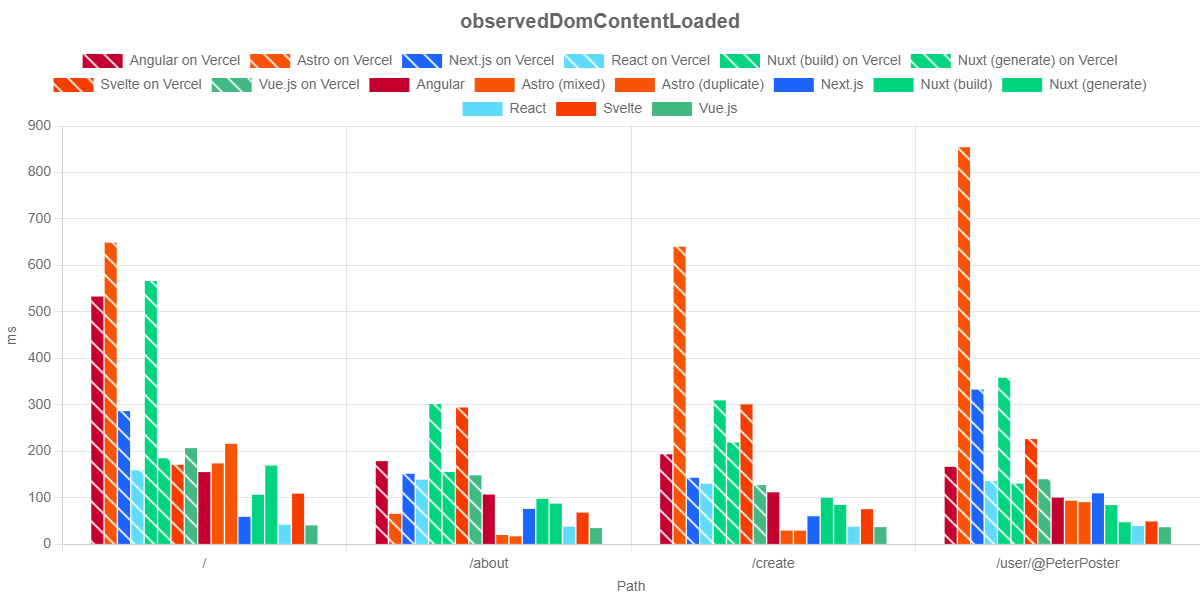
\includegraphics[width=\linewidth, keepaspectratio]{img/lighthouse-results/observedDomContentLoaded.png}
    \end{center}
    \caption{Observed DomContentLoaded}\label{subfig:LH:observedDomContentLoaded}
  \end{subfigure}
  \begin{subfigure}{0.49\linewidth}
    \begin{center}
      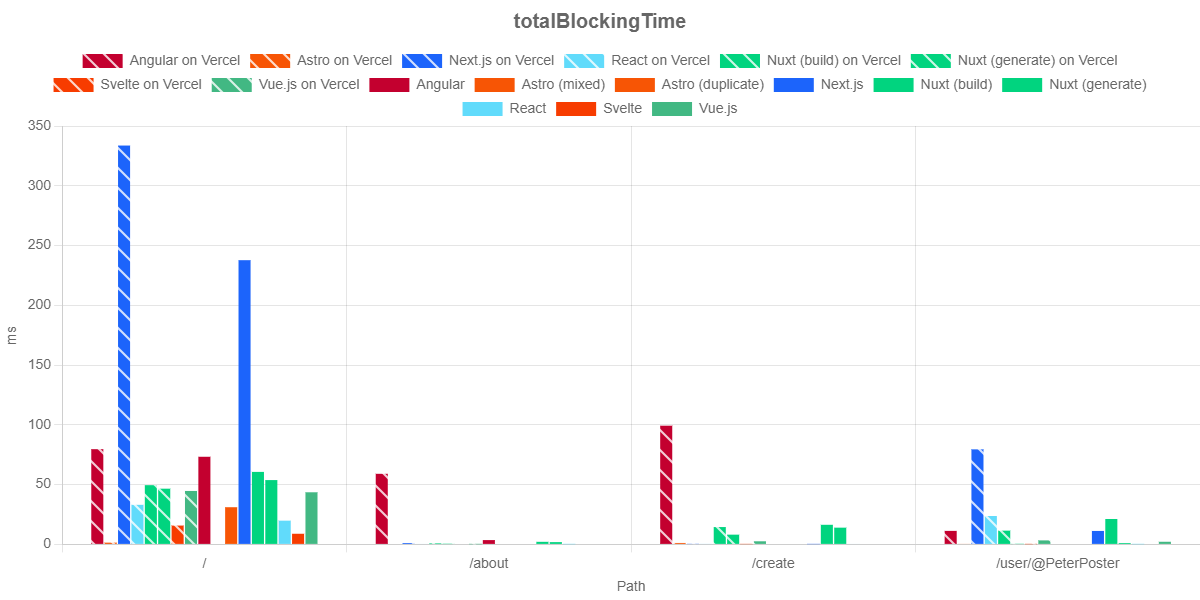
\includegraphics[width=\linewidth, keepaspectratio]{img/lighthouse-results/TBT.png}
    \end{center}
    \caption{\acrfull{tbt}}\label{subfig:LH:totalBlockingTime}
  \end{subfigure}
  \begin{subfigure}{0.49\linewidth}
    \begin{center}
      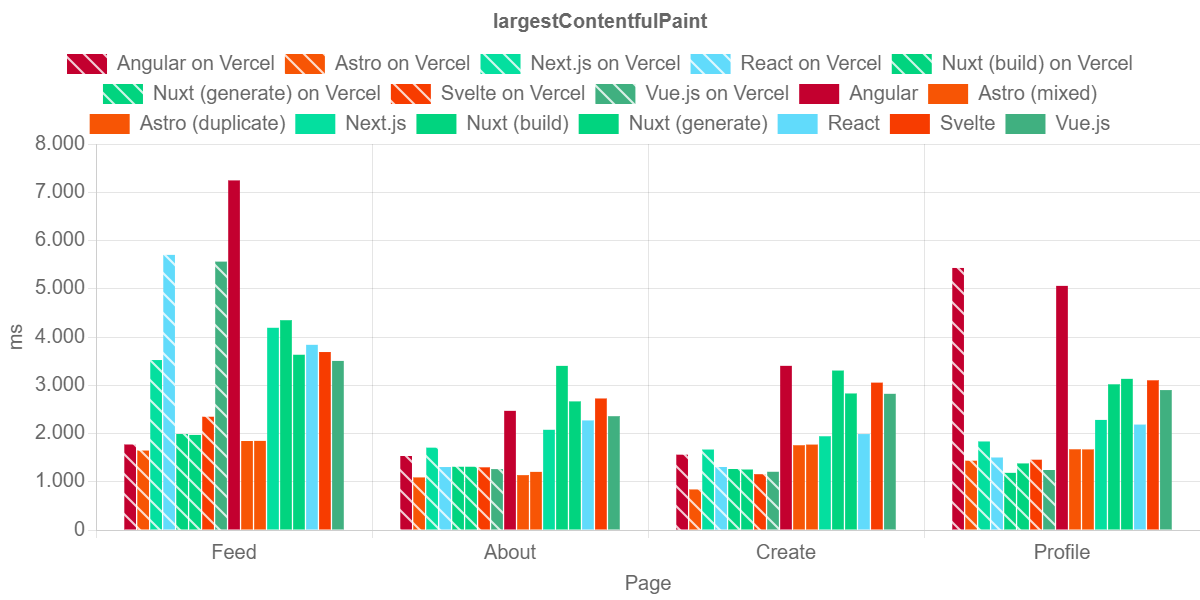
\includegraphics[width=\linewidth, keepaspectratio]{img/lighthouse-results/LCP.png}
    \end{center}
    \caption{\acrfull{lcp}}\label{subfig:LH:largestContentfulPaint}
  \end{subfigure}
  \begin{subfigure}{0.49\linewidth}
    \begin{center}
      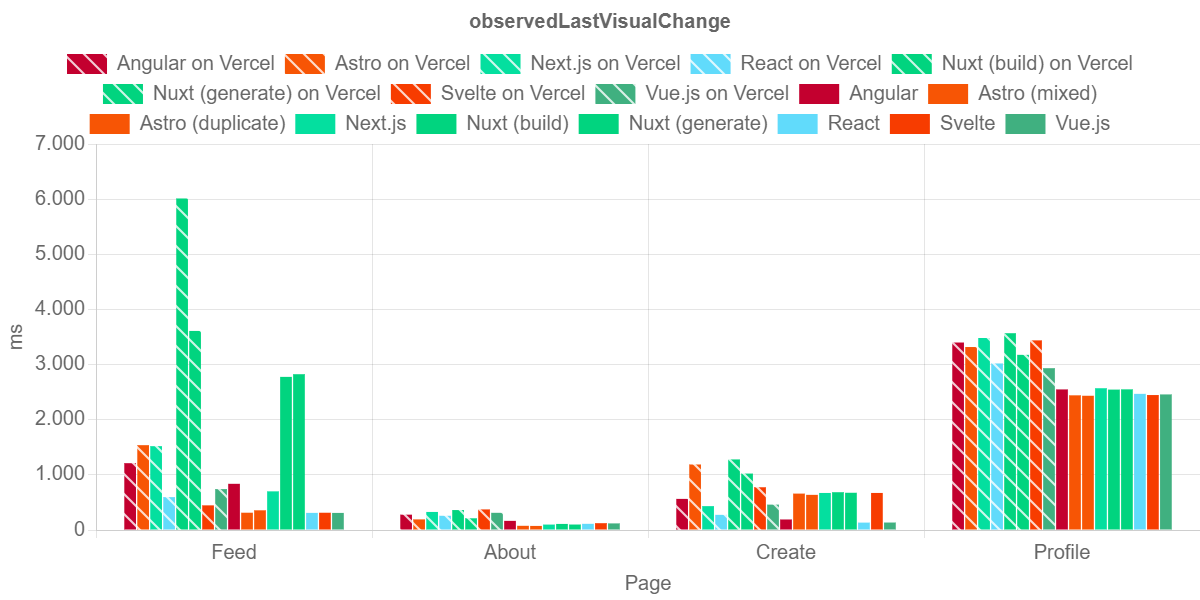
\includegraphics[width=\linewidth, keepaspectratio]{img/lighthouse-results/OLVC.png}
    \end{center}
    \caption{\acrfull{olvc}}\label{subfig:LH:observedLastVisualChange}
  \end{subfigure}
  \begin{subfigure}{0.49\linewidth}
    \begin{center}
      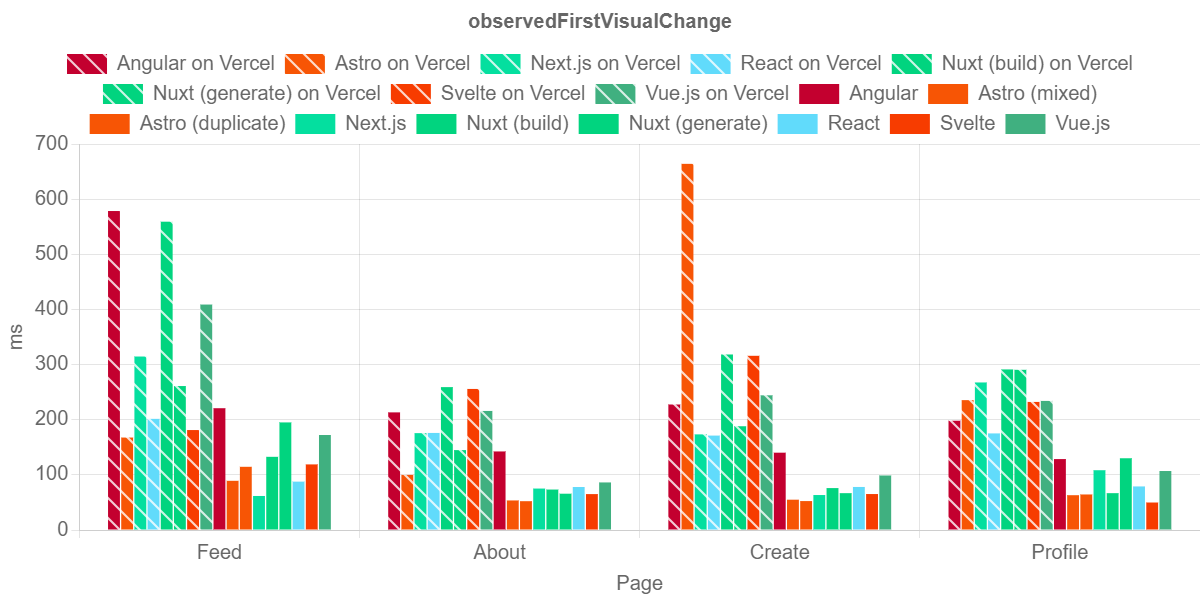
\includegraphics[width=\linewidth, keepaspectratio]{img/lighthouse-results/OFVC.png}
    \end{center}
    \caption{\acrfull{olvc}}\label{subfig:LH:observedLastVisualChange}
  \end{subfigure}
  \caption{Lighthouse test results in Google Chrome}\label{fig:lighthouseResults}
\end{figure}

\textbf{Page Load Time.} Next.js, Astro and Svelte are the leading frameworks in \acrshort{tbw} and Svelte, Next.js, Vue.js and especially Astro have fast results in their \acrshort{tti}.
In addition, Astro, Angular, Svelte, Nuxt and Vue.js stand out through little fluctuations in \acrshort{tti} across the four pages and the test repetitions.
The results of measurements for the \acrshort{tbt} also favor Astro and Svelte.
In contrast, Astro and Svelte perform poorly in DomContentLoaded and balanced LoadEventEnd (see figure \ref{fig:Playwright:loadEventEnd}).
These metrics are strengths of Vue.js, React and Nuxt.
The balanced LoadEventEnd is the difference between LoadEventEnd and the requestStart (see equation \ref{eq:balancedloadeventend}).
Vue.js and React are also the fastest frameworks in \acrshort{olvc}.
The \acrshort{ttfb} does not support a ranking of frameworks.
Instead, it is more dependent on the page content and the host, which influence the results more than the framework.
However, Astro, Next.js and Angular stand out through slow results in this metric.
The balanced LoadEventEnd highlights Vue.js and React positively, but also demonstrates a high dependency on the browser.

\vspace{-0.3cm}
\begin{equation}\label{eq:balancedloadeventend}
\mathit{loadEventEnd}_\mathit{balanced} = \mathit{loadEventEnd}_\mathit{raw} - \mathit{requestStart}
\end{equation}
\vspace{-0.2cm}

\textbf{Component Load Time.} The metrics for the component load time have similar characteristics.
The \acrshort{ofvc} of the applications are early in Astro, React and Next.js, which indicates a strength of React-based frameworks.
React, Vue.js and Angular also naturally have a short \acrfull{ovcd} (see figure \ref{fig:LH:OVCD}), which is unsurprising.
The \acrshort{ovcd} is defined as the time difference between \acrshort{ofvc} and \acrshort{olvc} (see equation \ref{eq:ovcd}).
The recordings of early \acrshort{dom} mutations are also very fast for Astro, Vue.js and React, whereas recordings are missing completely for Angular (see figure \ref{fig:Playwright:pageLoadMutations:total}).
This is most likely due to a faulty initialization of the MutationObserver that is responsible for recording mutation times.

\vspace{-0.8cm}
\begin{multline}\label{eq:ovcd}
  \mathit{observedVisualChangeDuration} =\\ \mathit{observedLastVisualChange} - \mathit{observedFirstVisualChange}
\end{multline}
% \vspace{0.0cm}

\textbf{Component Update Time.} In contrast, the measurements made for the component update times suggest clear rankings of the frameworks and of the used browsers (see figure \ref{fig:playwrightResults:total} and table \ref{tab:mutations:times}).
The times of the \acrshort{dom} mutations are quite similar to each other except in Mobile Safari and Desktop Safari.
In these browsers, Next.js is the slowest and Nuxt is the fastest framework.
Across all pages and frameworks, the ranking of browsers from fastest to slowest is Google Chrome, Microsoft Edge, Chromium, Mobile Chrome, Firefox, Mobile Safari and Desktop Safari.
This means that time budgets are most easily kept to in Google Chrome and hardest in Desktop Safari.
The ranking of frameworks is - from fastest to slowest - Nuxt, Angular, Vue.js, React, Astro/Svelte and Next.js.
In addition, Nuxt, Vue.js and Svelte are economical with \acrshort{dom} mutations after user interaction, whereas the other frameworks update the \acrshort{dom} after user interaction in more different ways.
This ranking can influence the choice of framework for user input heavy applications.
For this kind of application, Nuxt, Angular, Vue.js and React present themselves as the best choices relating to component update times.

\begin{figure}[!h]
  \centering
  \begin{subfigure}{0.49\linewidth}
    \begin{center}
      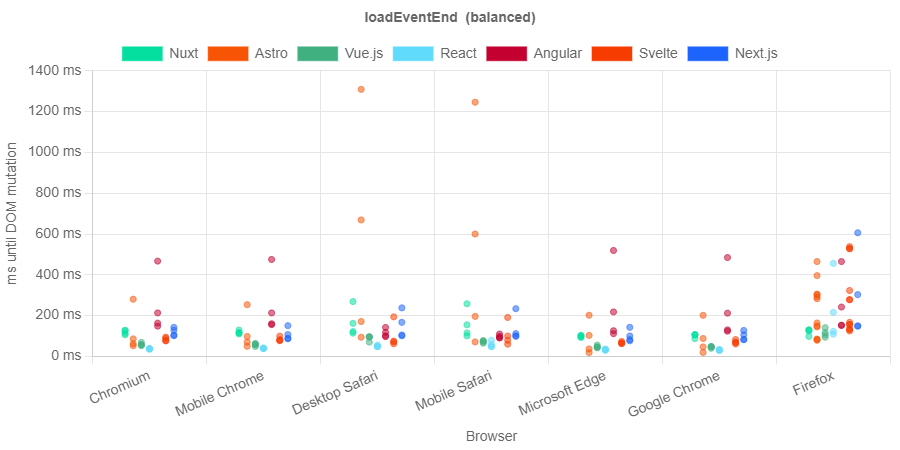
\includegraphics[width=\linewidth, keepaspectratio]{img/playwright-results/loadEventEnd_balanced/total.png}
    \end{center}
    \caption{Balanced loadEventEnd timings}
    \label{fig:Playwright:loadEventEnd}
  \end{subfigure}
  \begin{subfigure}{0.49\linewidth}
    \begin{center}
      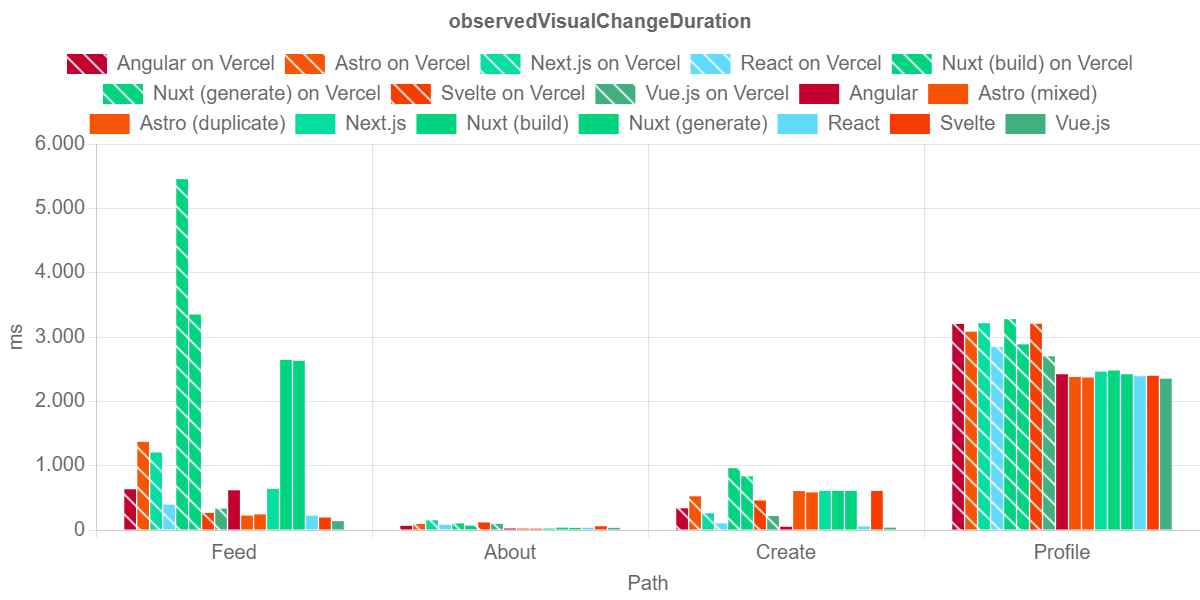
\includegraphics[width=\linewidth, keepaspectratio]{img/lighthouse-results/olvc-ofvc.png}
    \end{center}
    \caption{\acrfull{ovcd}}
    \label{fig:LH:OVCD}
  \end{subfigure}
  \begin{subfigure}{0.49\linewidth}
    \begin{center}
      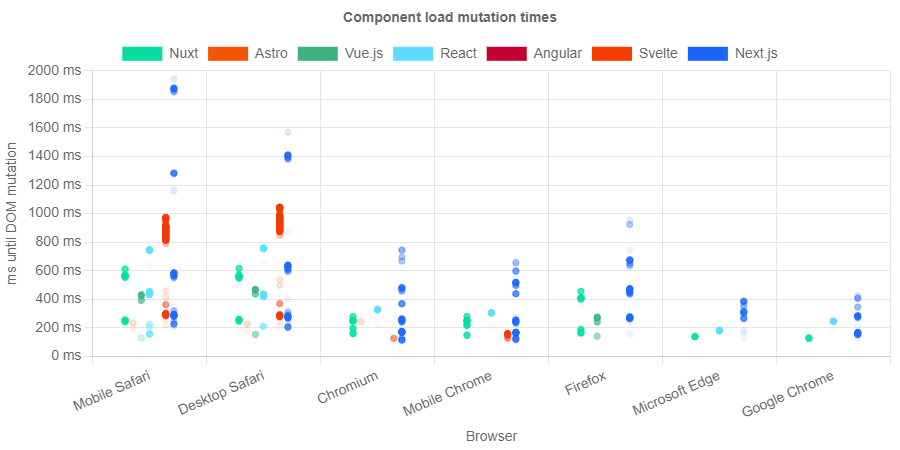
\includegraphics[width=\linewidth, keepaspectratio]{img/playwright-results/pageLoadMutations/total.png}
    \end{center}
    \caption{Component load mutation times}
    \label{fig:Playwright:pageLoadMutations:total}
  \end{subfigure}
  \begin{subfigure}{0.49\linewidth}
    \begin{center}
      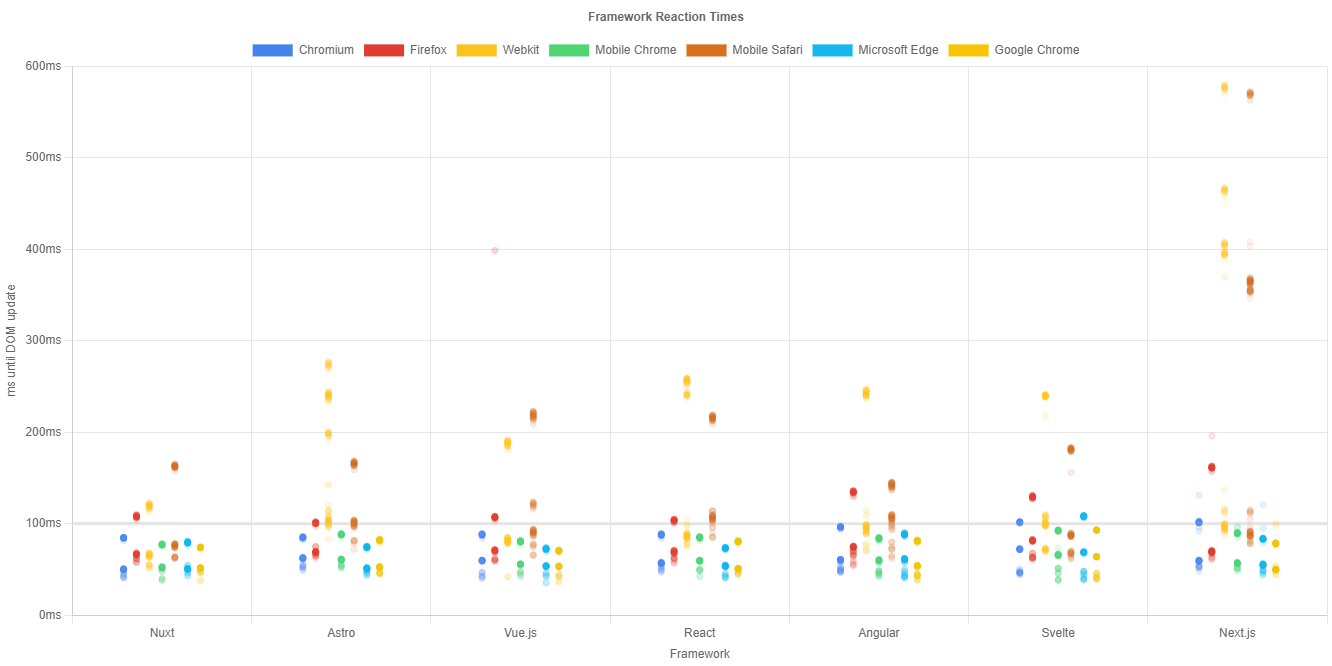
\includegraphics[width=\linewidth, keepaspectratio]{img/playwright-results/userActions_byUserAction/total.png}
    \end{center}
    \caption{Recorded \acrshort{dom} mutation timings after user actions}
    \label{fig:playwrightResults:total}
  \end{subfigure}
  \caption{}
\end{figure}

% DOM Mutation times state change
\begin{table}[h!]
  {\footnotesize
  \centering
  \begin{adjustbox}{angle=0}
    {
      \rowcolors{1}{lightgray!40!}{lightgray!40!}
      \begin{tabular}{|l|c|c|c|c|c|c|c|}
        \hline
        ~                                            & \textbf{Angular} & \textbf{Astro}                  & \textbf{Next.js}                & \textbf{Nuxt}          & \textbf{React}  & \textbf{Svelte} & \textbf{Vue.js} \\ \hline
\rowcolor{white}                                     & 44               & 51                              & 47                              & 39                     & 44              & 38              & 51              \\
\rowcolor{white}                                     & \textbf{69}      & \textbf{71}                     & \textbf{75}                     & \textbf{66}            & \textbf{58}     & \textbf{74}     & \textbf{77}     \\
\rowcolor{white} \multirow{-3}{*}{Chromium}          & 95               & 89                              & 108                             & 94                     & 85              & 95              & 104             \\ \hline
                                                     & 54               & 63                              & 59                              & 59                     & 54              & 60              & 52              \\
                                                     & \textbf{89}      & \textbf{99}                     & \textbf{142}                    & \textbf{83}            & \textbf{84}     & \textbf{94}     & \textbf{82}     \\
                 \multirow{-3}{*}{Firefox}           & 123              & 142                             & 235                             & 108                    & 181             & 129             & 103             \\ \hline
\rowcolor{white}                                     & 77               & \cellcolor{red!50}87            & 79                              & 51                     & 84              & 70              & 47              \\
\rowcolor{white}                                     & \textbf{123}     & \textbf{170}                    & \cellcolor{red!50}\textbf{304}  & \textbf{86}            & \textbf{169}    & \textbf{164}    & \textbf{136}    \\
\rowcolor{white} \multirow{-3}{*}{Desktop Safari}    & 172              & 270                             & \cellcolor{red!50}493           & 124                    & 280             & 283             & 200             \\ \hline
                                                     & 44               & 49                              & 47                              & 42                     & 44              & 45              & 46              \\
                                                     & \textbf{67}      & \textbf{69}                     & \textbf{94}                     & \textbf{61}            & \textbf{67}     & \textbf{81}     & \textbf{69}     \\
                 \multirow{-3}{*}{Mobile Chrome}     & 90               & 85                              & 143                             & 82                     & 82              & 116             & 89              \\ \hline
\rowcolor{white}                                     & 52               & 78                              & 73                              & 47                     & 67              & 56              & 52              \\
\rowcolor{white}                                     & \textbf{106}     & \textbf{154}                    & \textbf{196}                    & \textbf{110}           & \textbf{126}    & \textbf{126}    & \textbf{133}    \\
\rowcolor{white} \multirow{-3}{*}{Mobile Safari}     & 152              & 254                             & 372                             & 167                    & 183             & 208             & 206             \\ \hline
                                                     & 43               & 44                              & 46                              & 37                     & 41              & 40              & 40              \\
                                                     & \textbf{70}      & \textbf{64}                     & \textbf{73}                     & \textbf{61}            & \textbf{62}     & \textbf{74}     & \textbf{61}     \\
                 \multirow{-3}{*}{Microsoft Edge}    & 90               & 80                              & 134                             & 85                     & 75              & 102             & 79              \\ \hline
\rowcolor{white}                                     & 41               & 43                              & 41                              & \cellcolor{green!50}34 & 40              & 39              & 37              \\
\rowcolor{white}                                     & \textbf{62}      & \cellcolor{green!50}\textbf{57} & \textbf{69}                     & \textbf{60}            & \textbf{59}     & \textbf{64}     & \textbf{61}     \\
\rowcolor{white} \multirow{-3}{*}{Google Chrome}     & 84               & \cellcolor{green!50}72          & 99                              & 77                     & 77              & 89              & 77              \\ \hline
                 \hline
                                                     & 51               & 59                              & 56                              & 44                     & 53              & 50              & 46              \\
                                                     & \textbf{84}      & \textbf{98}                     & \textbf{136}                    & \textbf{75}            & \textbf{89}     & \textbf{97}     & \textbf{88}     \\
                 \multirow{-3}{*}{Browser Average}   & 115              & 142                             & 226                             & 105                    & 138             & 146             & 123             \\ \hline
\rowcolor{white}                                     & 45               & 48                              & 45                              & 35                     & 45              & 42              & 36              \\
\rowcolor{white}                                     & \textbf{69}      & \textbf{74}                     & \textbf{107}                    & \textbf{60}            & \textbf{75}     & \textbf{78}     & \textbf{70}     \\
\rowcolor{white} \multirow{-3}{*}{Weighted Browser Average}    & 94     & 104                             & 167                             & 80                     & 110             & 118             & 93              \\ \hline
      \end{tabular}

    }

    \end{adjustbox}

    \vspace{0.5cm}
      
    {\rowcolors{1}{lightgray!40!}{lightgray!40!}
    
      \begin{tabular}{|l|c|}
        \hline
        ~                                           & \textbf{Framework} \\ \hline
        \rowcolor{white}                            & minimum with framework in browser \\
        \rowcolor{white}                            & \textbf{average with framework in browser} \\
        \rowcolor{white} \multirow{-3}{*}{Browser}  & maximum with framework in browser \\ \hline \hline
                                                    & average of minima across browsers \\
                                                    & \textbf{total average across browsers} \\
                \multirow{-3}{*}{Browser Average}   & average of maxima across browsers \\ \hline
      \end{tabular}
    }
  \caption{Minimum, average and maximum of recorded mutation times after user input in milliseconds (fastest times are highlighted green, slowest red). Weights are based on browser usage quota \citep{browserUsage}.}
  \label{tab:mutations:times}
  }
\end{table}

\section{Summary}
% Rankings of frameworks
% Rankings of browsers
% Future work

The results of the study are inconclusive in relation to load times for both pages and components.
The measurements only show general advantages of single frameworks for the component update time.

Nuxt is the fastest framework in regards to component update time, whereas Next.js is the slowest.
Likewise, Google Chrome turns out to be the fastest browser for component updates
These updates are slowest in Desktop Safari.

However, test results fluctuate between repetitions. For this reason, future work should focus on making these results more reliable and statistically interpretable.
Reliability might be achieved through repetition of the study with more test runs and the inclusion of other hosting environments.
Additional pages might outline dependencies of the performance on the type of web page.
Continuations of this study could also expand the user actions to other interactions than filling a form, for instance navigation between pages.

This study also revealed that the used algorithms for start and end of the recording are suboptimal for the goals. 
% Solutions to problems within this study should lead to a better initialization algorithm and end of recording \acrshort{dom} mutations.
Therefore, some mutations are currently not recorded at all and the ending of the time frame for recording is manually set.
For these reasons, early mutations (fast loading components), slow mutations (slow loading components) and periodically mutating components, e.g. a digital clock, cannot be recorded properly.

\pagebreak

\appendix

% \lstlistoflistings

% \listoffigures

\rowcolors{1}{white}{white}
% \glsaddall
\printnoidxglossary[
  type=\acronymtype,
  nonumberlist,
  nogroupskip,
  % style=long
]

% \nocite{*}
\bibliography{sources}{}

\textbf{Github repository}: All code and additional material can be found under \url{https://github.com/andreasnicklaus/master}.

% \listoftables

\end{document}